\documentclass{article}

%Margins
\usepackage[margin=1in]{geometry}


%Float & Graphics 
\usepackage{float}
\usepackage{graphicx}

%Chemistry Equations
\usepackage [version = 3] {mhchem}

%Document
\begin{document}
%Title Page 
\begin{titlepage}
\title{The Effects of a change in Concentration and Temperature on the Iodine Clock Reaction Between $\ce{KIO_3}_{(l)}$, and $\ce{Na_{2}S_{2}O_{5}}_{(l)}$}
\author{Abhishek Sreekanth}
\date{4-28-2015}
\maketitle
\thispagestyle{empty}
\end{titlepage}
\setcounter{page}{1}

%Sections
\section*{Abstract} %Abstract 
The purpose of this experiment was to determine the Rate Law, and Activation Energy, in the reaction between Potassium Iodate, $\ce{KIO_3}_{(l)}$, and Sodium Metabisulfite, $\ce{Na_{2}S_{2}O_{5}}_{(l)}$, by comparing their relative reaction rates at two different concentrations and temperatures. After testing a decrease in concentration of reactants, by diluting them by hand, and testing an increase in temperature of the reaction. The rate laws for the two reactions were calculated, and from the rate laws the Activation Energy of this reaction was found. 
\pagebreak
\section*{Introduction} %Introduction
\subsection*{Purpose} %Purpose 
The purpose of this experiment was to determine the Rate Law, and Activation Energy, in the reaction between Potassium Iodate, $\ce{KIO_3}_{(l)}$, and Sodium Metabisulfite, $\ce{Na_{2}S_{2}O_{5}}_{(l)}$, by comparing their relative reaction rates at two different concentrations and temperatures.
\subsection*{Background}%Background
The rate of a chemical reaction is a measure of how fast the reaction occurs. A reaction with a fast rate has a relatively large amount of molecules reacting to form products in a given time. And a reaction with a slow rate has a relatively small amount of molecules reacting to form products in a given time (Tro, 2007). \\\\
\noindent
The rate of a chemical reaction is heavily dependent on the concentration of the products and reactants. To measure the rate of a reaction, the concentration of at least one of the products or reactants must be known. Over time, the reactant concentration decreases in a reaction, and the product concentration increases. This occurs because products are formed, by the usage of the reactants. This process, showing the reaction between Hydrogen and Iodine, is illustrated in Figure 1 below (Tro, 2007). 
%Graph Illustrating concentration over time
\begin{figure}[H]
	\centering
	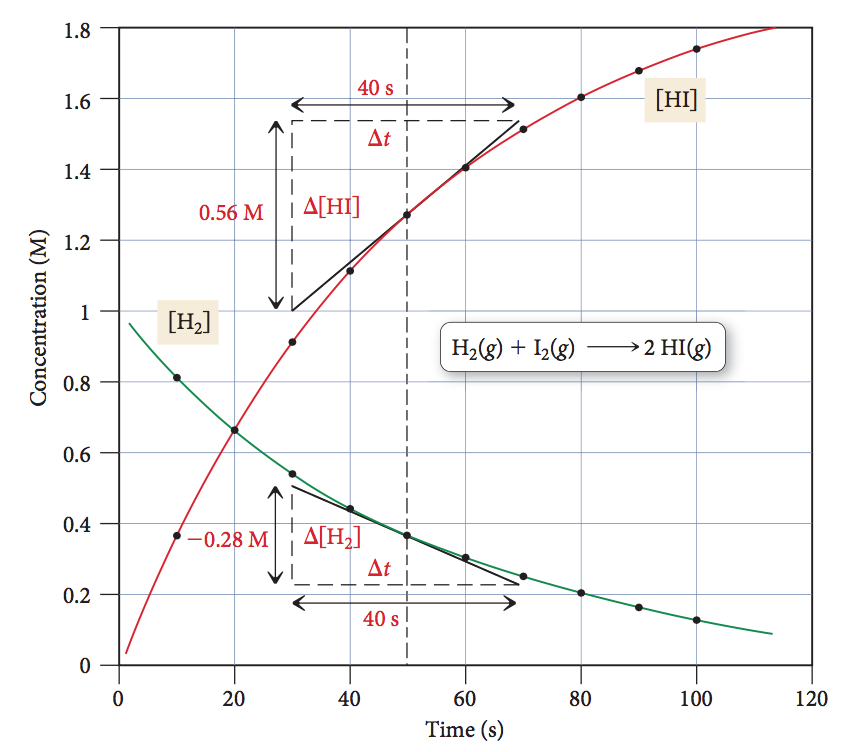
\includegraphics{1.png}
	\caption{Concentration over time for the reaction between Hydrogen and Iodine}
\end{figure}
\pagebreak %Pagebreak 
\noindent
Knowledge of reaction rates would enable greater profits to be acquired in manufacturing. By knowing how fast or how slow a reaction occurs, and what conditions affect that rate, conditions to maximize profit, by creating and selling more product, can be created. \\\\
\noindent
Activation Energy is the minimum amount of energy required to cause a reaction to occur. Thus, activation energy is present in all chemical reactions. Activation energy can be thought of as a barrier reactants need to overcome, to form a new product. To form a new product these reactants need to not only have enough kinetic energy, but they also need to collide in a proper orientation. If reactants collide with enough kinetic energy, and with a proper orientation, they will have been successful in forming a new product. The greater the activation energy, the longer it takes a reaction to occur (chemwiki.ucdavis.edu). \\\\
Knowledge of the Activation Energy of a reaction has many practical purposes. By knowing how much energy a reaction requires for it to occur, companies can maximize profits by only expending that amount of energy. Companies can save money energy bills by using less heat, to still get the product at the same speed. Knowledge of Activation Energy in conjunction with a knowledge of catalysts, can help companies maximize profits. Catalysts increase the speed of a chemical reaction, by lowering its activation energy. By having an understanding of how Catalysts work, companies would be able to maximize profit by producing a product more quickly, and capitalizing on the sales. \\\\
An Iodine Clock Reaction is a discontinuous reaction that when completed, will produce a black/blue colored solution. A discontinuous reaction is a reaction in which the rate cannot be directly observed and measured, rather it is more feasible to measure the reaction to a point where an observable change has occurred. For example, measuring the time it takes for the Iodine Clock Reaction to go black. \\
\begin{figure}[H]
	\centering
	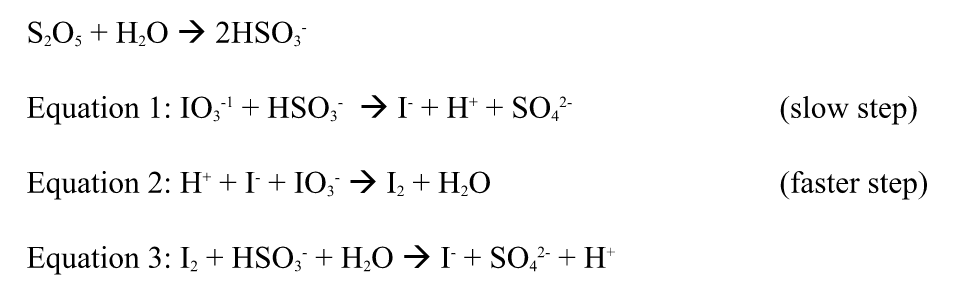
\includegraphics{2.png}
	\caption{Reaction Mechanism for an Iodine Clock Reaction}
\end{figure}
\noindent
The figure above shows a reaction mechanism for an Iodine Clock Reaction. In equation one, which is the first step of the reaction, Iodide ions are formed. This step is also known as the slow step. The slow step is the rate determining step of the reaction, as the reaction can't go faster than it's slowest step. Then in equation two, the iodate is turned into Iodine, however this step occurs too quickly to observe, so until all of the bimetasulfate is reacted, there is no observable change. \\\\
In a study conducted by Antonio C. Lasaga, from Yale University's department of Chemistry, The Activation Energies and Rates were measured to better understand the transformations of the earth. The results of these observations and calculations were then published. It was concluded that the rate of a species is related to its steady state of its system. Lasaga's study focused on the chemical kinetics of geochemistry, and developed the results in a geological context. Due to the fact that Lasaga's study only covered the geological realm, and had concluded that there were relationships between reaction rates and temperature and pressure, this experiment was conducted (Lasaga, Antonio, 1981). \\\\
This experiment was conducted to explore the Chemical Kinetics of the Iodine Clock Reaction, and to further explore the subjects in a more pragmatic setting. The results of this study can be applied on a commercial scale, to determine what amount, and in what conditions, certain reactions must take place to yield the most product. The results of this experiment can also be further explored upon in other fields of study as well. \\\\
The independent variables of this experiment were temperature and concentration, and the dependent variable was the reaction rate. 
\subsection*{Hypothesis}%Hypothesis
If a decrease in concentration causes a decrease in the rate of a reaction, and an increase in temperature causes an increase in the rate of a reaction, then the overall rate of the reaction between Potassium Iodate and Sodium Metabisulfite will decrease but its comparative rates will increase. 
\subsection*{Safety Information}%Safety Information
Safety is paramount, and good laboratory practices should not only be informed, but also practiced. The risk of burn was apparent, all throughout the experiment. Simple measures must be taken to prevent any sort of burn injuries. The hot-plates used, and hot beakers should be stationed at an area, away from foot traffic. Proper equipment should be used to touch and move the hot equipment, and lastly, safety googles must be worn at all times, in case of splattering.
\section*{Materials} %Materials
\begin{enumerate}
\item 50 mL Burette (2) \\
\item 250 mL Beaker (2)\\
\item 400 mL Beaker (2)\\
\item 140 mL Beaker	(4) \\
\item Burette stand (1) \\ 
\item Hot Plate (2) \\
\item	Timer (1) \\ 
\item	Stirring rod  (1) \\
\item	Thermometer (1) \\
\item	Tong (1) \\
\item	Paper (1) \\
\item	Pencil (1) \\
\item Weighing Dish (1) \\
\item	Scale (1) \\
\item15.0 mL \ce{KIO_{3}_{(l)}} (apx.) \\
\item 46.2 mL \ce{H_{2}O_{(l)}} (apx.) \\
\item 9.0 mL Starch Solution (apx.) \\
\item 3.0 mL $\ce{Na_{2}S_{2}O_{5}}_{(l)}$ (apx.) \\
\end{enumerate}

\section*{Methods}%Methods 
\subsection*{Calculating the Rate Expression} %Rate Exp 
\begin{eqnarray*}
Rate &=& K[A]^{a}[B]^{b} \\\\
\frac{Rate_{2}}{Rate_{1}} &=& \frac{K_{2}[A_{2}]^{a}[B_{2}]^{b}}{K_{1}[A_{1}]^{a}[B_{1}]^{b}} \\\\
\frac{Rate_{2}}{Rate_{1}} &=& \left[\frac{A_{2}}{A_{1}}\right]^a \\\\
a &=& \log_{\left[\frac{A_{2}}{A_{1}}\right]} \left(\frac{Rate_{2}}{Rate_{1}}\right) 
\end{eqnarray*}
To find the b value, repeat the same process, except replace the [A]'s and a's with [B] and b. 

\subsection*{Calculating the Rate Constant} %Rate Constant 
\begin{eqnarray*}
K &=& \frac{Rate}{[A]^{a}[B]^{b}}
\end{eqnarray*}

\subsection*{Calculating the Activation Energy} %Activation Energy 
To calculate the activation energy of the reaction, the Arrhenius equation, as shown below must be used:
\begin{eqnarray*}
\ln \left(\frac{K_1}{K_2}\right) &=& \frac{E_a}{R} \left(\frac{1}{T_2} - \frac{1}{T_1}\right)
\end{eqnarray*} \\
Where K is the rate constant, $E_a$ is the activation energy, R is the noble gas constant, and T is the temperature of the reaction. 
\section*{Procedure} %Procedure
2.5 mL of Potassium Iodate was poured into a 50 mL beaker containing 7.5 mL of water to create solution one. Then, 1.5 mL of a Starch Solution, .5 mL of Sodium Metabisulfate, and 2 mL distilled water was poured into a 50 mL beaker to create solution 2. Solution 1 was then poured into solution 2, and the time it took for the solution to change color was recorded. \\\\
The concentration of the Potassium Iodate solution had to be decreased to 0.04 M. It was calculated that $\frac{0.0036g}{2.5mL \ce{H_2O}}$ of Potassium Iodate created a 0.04M solution. Therefore, 0.0036g of \ce{KIO_3} was measured and poured into a 50mL beaker. Then, 2.5 mL of water was poured into the same 50mL beaker. The mixture was stirred vigorously for approximately one minute. After the new \ce{KIO_3} solution was created, the above process was followed, to form Solution 1 and 2, and to measure the time it took for the two solutions to change color. \\\\
The concentration of the Sodium Metabisulfate solution had to be decreased to 0.04 M. It was calculated that $\frac{0.038g}{0.5mL \ce{H_2O}}$ of Sodium Metabisulfate created a 0.04 M solution. Therefore, 0.038g of Sodium Metabisulfate was measured and poured into a 50mL beaker. Then, 0.5 mL of water was poured into the same 50mL beaker and the mixture was stirred vigorously for approximately one minute. After the 0.04 M solution of Sodium Metabisulfate was created, the above process of creating solution 1 and 2 was followed, and the time it took for the two solution to change color was measured.  \\\\
The 3 processes mentioned above were repeated again, to measure the rate of the reaction at a temperature of $46^o C$. After all the solutions were prepared, two heat plates were initially heated. Solution 1 was transferred into a 140 mL beaker and placed on top of the heat plates. Solution 2 was also placed on a hot plate, however, it remained in a 50 mL beaker. A thermometer was placed inside each of the beakers and the temperature was measured to approximately $48^o C$. After the two solution reached that temperature they were removed from hot plates and placed onto a flat surface. When both solution reached a temperature of $46^o C$, solution 2 was poured into solution 1 and the time it took for the two solutions to change color was measured. 
\section*{Results} %Results
\subsection*{Raw Data} %Raw Data
%Table 1
\begin{table}[H]
	\centering
	\title{Iodine Clock Reaction at $25^o C$} \\
	\begin{tabular}{c | c | c | c | c} \\
		Trail & \ce{KIO_{3}_{(l)}} & \ce{Na_{2}S_{2}O_{5}_{(l)}} & Time & Rate \\ \hline
		1 & 0.2 & 0.2 & 10.03 & 1 \\
		2 & 0.04 & 0.2 & 52.69 & 0.19 \\
		3 & 0.2 & 0.04 & 57.27 & 0.18 \\
	\end{tabular}
	\caption{Data for reaction at $25^o C$}
	\label{tab:1} 
\end{table} 
%Table 2	
\begin{table}[H]
	\centering
	\title{Iodine Clock Reaction at $45^o C$}  \\
	\begin{tabular}{c | c | c | c | c} \\
		Trail & \ce{KIO_{3}_{(l)}} & \ce{Na_{2}S_{2}O_{5}_{(l)}} & Time & Rate \\ \hline
		1 & 0.2 & 0.2 & 29.68 & 1 \\
		2 & 0.04 & 0.2 & 66.18 & 0.45 \\
		3 & 0.2 & 0.04 & 71.94 & 0.41 \\
	\end{tabular}
	\caption{Data for reaction at $45^o C$}
	\label{tab:2}
\end{table}
%Table 3
\begin{table}[H]
	\centering
	\title{Order of Reactions and their K values }  \\
	\begin{tabular}{c | c | c | c} \\
		Temperature & a value & b value & K value \\ \hline
		$25^o C$ & 1.03 & 1.06 & 28.90 \\ 
		$45^o C$ & 0.50 & 0.55 & 5.42 \\ 
	\end{tabular}
	\caption{a, b, and K values of the reactions}
	\label{tab:3}
\end{table} 
\subsection*{Important Results}%Important Results
The order with respect to \ce{KIO_3} for the $25^o C$ reaction was calculated to 1.03, and was calculated to 0.50 for the $45^o C$ reaction. The order with respect to \ce{Na_{2}S_{2}O_{5}} for the $25^o C$ reaction was calculated to 1.06, and was calculated to 0.55 for the $45^o C$ reaction. The rate constant for the $25^o C$ reaction was calculated to 28.90, and was calculated to 5.42 for the $45^o C$ reaction. Lastly, the activation energy for this reaction was calculated to -6507.19 J. 
\subsection*{Calculations}%Calculations
\subsubsection*{Diluting \ce{KIO_3}}
\subsubsection*{Diluting \ce{Na_{2}S_{2}O_{5}}}
\subsubsection*{Calculating Orders of Reaction for $25^o C$ Reaction} %25 rxn
\begin{eqnarray*}
	\frac{0.19}{1} &=& \frac{[0.04]^{a}[0.2]^{b}}{[0.2]^{a}[0.2]^{b}} \\\\
	0.19 &=& 0.2^{a}\\\\
	\log_{0.2} 0.19 &=& a \\\\
	a &=& 1.03 \\\\
	\frac{0.18}{1} &=& \frac{[0.2]^{a}[0.04]^{b}}{[0.2]^{a}[0.2]^{b}} \\\\
	0.19 &=& 0.2^{b} \\\\
	\log_{0.2} 0.18 &=& b \\\\
	b &=& 1.06 
\end{eqnarray*}
\subsubsection*{Calculating K-value for the $25^o C$ Reaction}
\begin{eqnarray*}
	\frac{1}{[0.2]^{1.03}[0.2]^{1.06}} &=& 28.90 \\\\
	K &=& 28.90 
\end{eqnarray*}
\subsubsection*{Calculating Orders of Reaction for $45^o C$ Reaction}
\begin{eqnarray*}
	\frac{0.45}{1} &=& \frac{[0.04]^{a}[0.2]^{b}}{[0.2]^{a}[0.2]^{b}} \\\\
	0.45 &=& 0.2^{a} \\\\
	\log_{0.2} 0.45 &=& a \\\\
	a &=& 0.50 \\\\
	\frac{0.41}{1} &=& \frac{[0.2]^{a}[0.04]^{b}}{[0.2]^{a}[0.2]^{b}} \\\\
	0.41 &=& 0.2^{b} \\\\
	\log_{0.2} 0.41 &=& b \\\\
	b &=& 0.55 
\end{eqnarray*}
\subsubsection*{Calculating K-value for the $45^o C$ Reaction}
\begin{eqnarray*}
	\frac{1}{[0.2]^{0.5}[0.2]^{0.55}} &=& 5.42 \\\\
	K &=& 28.90
\end{eqnarray*}
\subsubsection*{Calculating Activation Energy} 
\begin{eqnarray*}
	\ln \left(\frac{28.90}{5.42}\right) &=& \frac{E_a}{8.31} \left(\frac{1}{318} - \frac{1}{298} \right)\\
	1.67 &=& \frac{E_{a}}{8.31}\left(-2.11*10^{-4}\right) \\
	-7912.79 &=& \frac{E_a}{8.31} \\
	E_a &=& -6567.19 J
\end{eqnarray*}
\section*{Discussion}%Discussion
\subsection*{Conclusion}
The hypothesis states that a decrease in concentration and an increase in temperature of a reaction will cause an overall decrease in the rate of a reaction, however an increase in the comparative rates. The results of the experiment support the hypothesis. At each individual temperature, the rates of the reaction decreased as the concentration decreased. The overall rates of the reaction decreased, as indicated by the decrease in the reaction's K-value. However, when the concentration was held constant and the temperature increased, the rate of the individual reactions increased. Table 1 and Table 2 illustrate show that the comparative rates, when concentration is held constant, increases in the reaction. Table 3 shows that the overall rate of the reaction, indicated by the K-value, decreased, even with the increase in temperature. \\\\
In conclusion, this experiment supports the hypothesis that while the overall rate of the reaction decreases, the comparative rates, the rates when concentration is held constant, increases. 
\subsection*{Experimental Error} %Experimental Error 
This experiment, like all experiment, was associated with errors. First, no measuring device is perfectly precise, and will consequently carry a certain uncertainty value. Next, the method used to decrease the concentration of the reactants had a lot of errors associated with it. One, the values that were calculated are very small, and the most precise machines were not used. There could have been a greater amount of reactant added to the solution, due to the nature of the calculations. The weighing dishes could have been contaminated with particles, that could have caused a deficit in reactant used to create the new solution. The method used to measure the heat of the solutions was not the most precise. The thermometer could have measured the temperature of the glass vs the temperature of the water. The thermometer could have also been affected by the draft created from moving the beakers off of the glass and onto a flat surface, to cool down the two solutions. Lastly, by transferring the solution from a 50 mL beaker to a 140 mL beaker, some of the solution could have been lost, causing the data to be manipulated. 
\subsection*{Improvements} %Improvements 
To reduce the listed errors, alternate methods should be used. The most precise lab materials should be used, to reduce all the listed errors. Electronic scales, or computerized scales could have been used to drastically reduce the margin for error on smaller measurements. The two solutions could have been in a heated chamber, instead of a hot plate, and should have been insulated so that drafts wouldn't affect the thermometer's readings. And lastly the transfer of final solutions, from one beaker to another, should be limited as that would reduce the amount of solution lost, and would give the most accurate data. 
\end{document}
